\section{Logical view}

Som beskrevet i view beskrivelser på forrige side består logical viewet af designoverview-, sekvens-, statemachines og klassediagrammer. Til at lave diagrammerne anvendes applikationsmodellen.

\subsection{Applikationsmodel}
Applikationsmodellen anvendes til at udvikle diagrammerne tilhørende logical view. Med applikationsmodellen tages der udgangspunkt i use cases beskrevet i kravspecifikationen og domain modellen, se figur \ref{fig:domain_model}.
  
Ud fra domain modellen identificeres de overordnede klasser der skal bruges til de forskellige use cases. Når de overordnede klasser er identificeret beskrives hvordan de kommunikerer via desginoverview og sekvensdiagrammer. Herefter laves statemachines med de fundne klasser og til sidst udarbejdes klassediagrammer.


\subsection{Use case 1}

Brugeren tilslutter batteriet. Dronen indikere via en rød LED at der ikke er oprettet forbindelse. Dronen opretter nu forbindelse til server og satellitter til GPS position. Efter nogle sekunder ser brugeren at den røde LED er slukket og en grøn LED er tændt. Dronen er nu klar til at modtage flyveinformationer fra bruger og derved klar til at flyve.

\vspace{-5pt}
%kommentar
\begin{figure}[H]
	\centering
	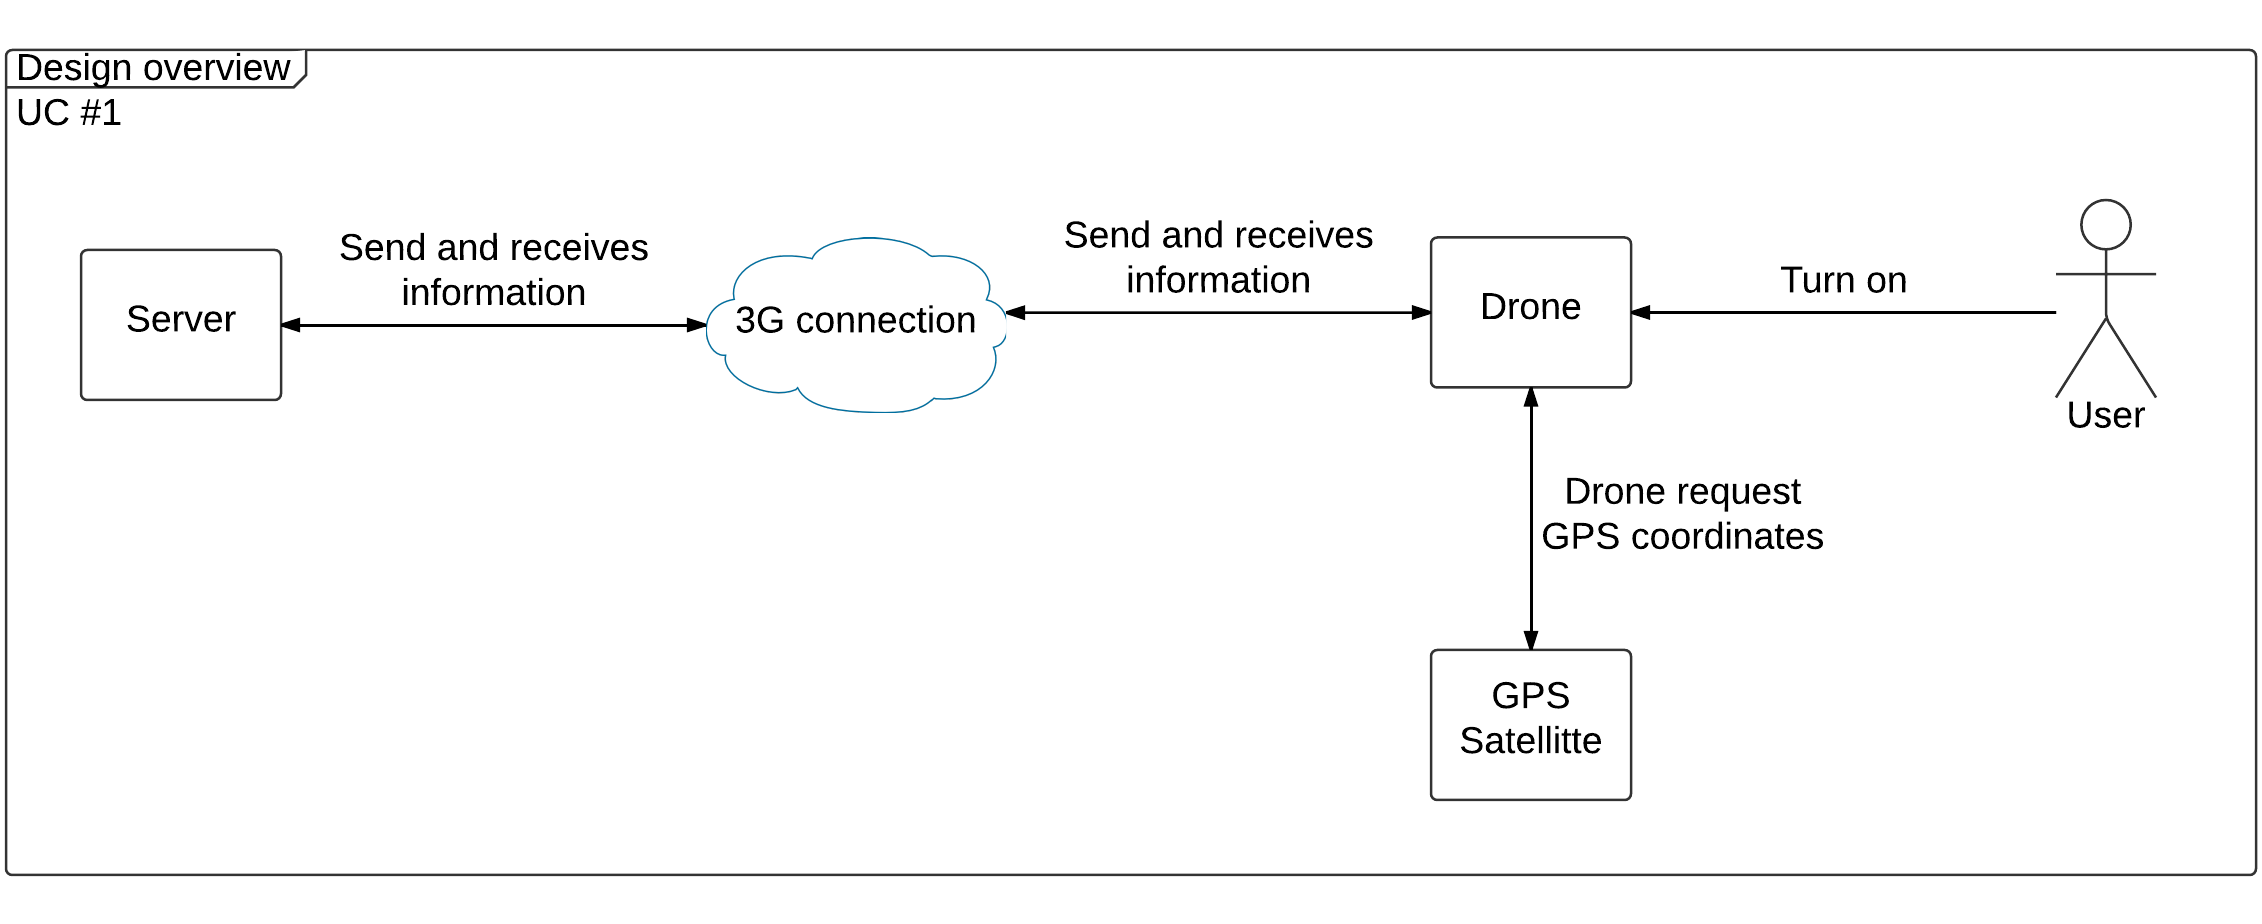
\includegraphics[width=1\textwidth]{Billeder/design_overview/design_overview_UC1.png}
	\vspace{-1cm}
	\caption{Design overview iteration 1}
	\label{fig:design_overview_it1}
\end{figure}




